\begin{figure}[H]

\centering
\tikzset{every picture/.style={line width=0.75pt}} %set default line width to 0.75pt        

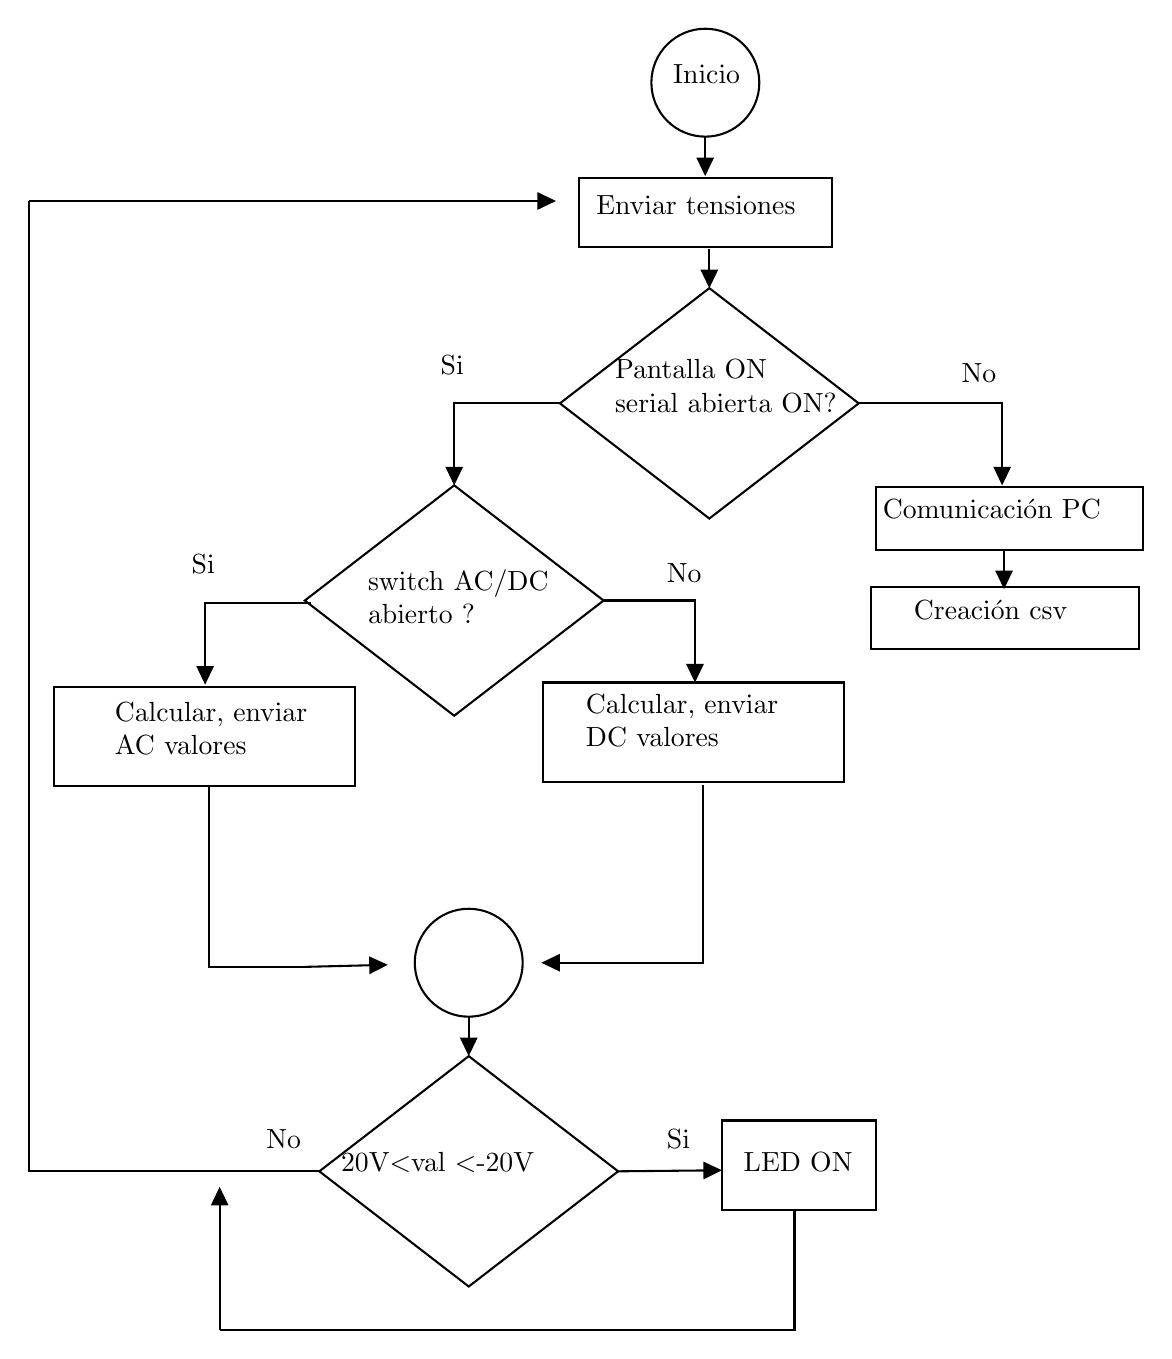
\begin{tikzpicture}[x=0.75pt,y=0.75pt,yscale=-1,xscale=1]
%uncomment if require: \path (0,736); %set diagram left start at 0, and has height of 736

%Flowchart: Connector [id:dp7813495520702245] 
\draw   (320,81) .. controls (320,66.64) and (331.64,55) .. (346,55) .. controls (360.36,55) and (372,66.64) .. (372,81) .. controls (372,95.36) and (360.36,107) .. (346,107) .. controls (331.64,107) and (320,95.36) .. (320,81) -- cycle ;
%Straight Lines [id:da8847526091998554] 
\draw    (345.92,107) -- (345.92,123) ;
\draw [shift={(345.92,126)}, rotate = 270] [fill={rgb, 255:red, 0; green, 0; blue, 0 }  ][line width=0.08]  [draw opacity=0] (8.93,-4.29) -- (0,0) -- (8.93,4.29) -- cycle    ;
%Flowchart: Process [id:dp3892985602062795] 
\draw   (285,127) -- (407,127) -- (407,160) -- (285,160) -- cycle ;
%Flowchart: Decision [id:dp21596588394867888] 
\draw   (347.92,180) -- (419.9,235.5) -- (347.92,291) -- (275.94,235.5) -- cycle ;
%Straight Lines [id:da7204417446380422] 
\draw    (347.92,161) -- (347.92,177) ;
\draw [shift={(347.92,180)}, rotate = 270] [fill={rgb, 255:red, 0; green, 0; blue, 0 }  ][line width=0.08]  [draw opacity=0] (8.93,-4.29) -- (0,0) -- (8.93,4.29) -- cycle    ;
%Straight Lines [id:da451260237829443] 
\draw    (489,256) -- (489,272) ;
\draw [shift={(489,275)}, rotate = 270] [fill={rgb, 255:red, 0; green, 0; blue, 0 }  ][line width=0.08]  [draw opacity=0] (8.93,-4.29) -- (0,0) -- (8.93,4.29) -- cycle    ;
%Straight Lines [id:da49582350632228556] 
\draw    (225,256) -- (225,272) ;
\draw [shift={(225,275)}, rotate = 270] [fill={rgb, 255:red, 0; green, 0; blue, 0 }  ][line width=0.08]  [draw opacity=0] (8.93,-4.29) -- (0,0) -- (8.93,4.29) -- cycle    ;
%Straight Lines [id:da9013438330772021] 
\draw    (153.04,507) -- (190,506.08) ;
\draw [shift={(193,506)}, rotate = 178.57] [fill={rgb, 255:red, 0; green, 0; blue, 0 }  ][line width=0.08]  [draw opacity=0] (8.93,-4.29) -- (0,0) -- (8.93,4.29) -- cycle    ;
%Straight Lines [id:da797473974800426] 
\draw    (330,505) -- (270,505) ;
\draw [shift={(267,505)}, rotate = 360] [fill={rgb, 255:red, 0; green, 0; blue, 0 }  ][line width=0.08]  [draw opacity=0] (8.93,-4.29) -- (0,0) -- (8.93,4.29) -- cycle    ;
%Straight Lines [id:da006314317293441896] 
\draw    (232,531) -- (232,547) ;
\draw [shift={(232,550)}, rotate = 270] [fill={rgb, 255:red, 0; green, 0; blue, 0 }  ][line width=0.08]  [draw opacity=0] (8.93,-4.29) -- (0,0) -- (8.93,4.29) -- cycle    ;
%Straight Lines [id:da9058055932314646] 
\draw    (303.98,605.5) -- (351,605.03) ;
\draw [shift={(354,605)}, rotate = 179.43] [fill={rgb, 255:red, 0; green, 0; blue, 0 }  ][line width=0.08]  [draw opacity=0] (8.93,-4.29) -- (0,0) -- (8.93,4.29) -- cycle    ;
%Straight Lines [id:da1932315478192832] 
\draw    (489.92,306) -- (489.92,322) ;
\draw [shift={(489.92,325)}, rotate = 270] [fill={rgb, 255:red, 0; green, 0; blue, 0 }  ][line width=0.08]  [draw opacity=0] (8.93,-4.29) -- (0,0) -- (8.93,4.29) -- cycle    ;
%Straight Lines [id:da6050013822698619] 
\draw    (20,138) -- (271,138) ;
\draw [shift={(274,138)}, rotate = 180] [fill={rgb, 255:red, 0; green, 0; blue, 0 }  ][line width=0.08]  [draw opacity=0] (8.93,-4.29) -- (0,0) -- (8.93,4.29) -- cycle    ;
%Shape: Right Angle [id:dp24954692627046726] 
\draw   (419.9,235.5) -- (489,235.5) -- (489,256) ;
%Flowchart: Process [id:dp33592140600780107] 
\draw   (428,276) -- (557,276) -- (557,306) -- (428,306) -- cycle ;
%Shape: Right Angle [id:dp2914826540765745] 
\draw   (275.94,235.5) -- (225,235.5) -- (225,256) ;
%Flowchart: Decision [id:dp9064156706798434] 
\draw   (225,275) -- (296.98,330.5) -- (225,386) -- (153.02,330.5) -- cycle ;
%Straight Lines [id:da6126735924115385] 
\draw    (341,351) -- (341,367) ;
\draw [shift={(341,370)}, rotate = 270] [fill={rgb, 255:red, 0; green, 0; blue, 0 }  ][line width=0.08]  [draw opacity=0] (8.93,-4.29) -- (0,0) -- (8.93,4.29) -- cycle    ;
%Shape: Right Angle [id:dp7943090498770735] 
\draw   (296.98,330.5) -- (341,330.5) -- (341,351) ;
%Straight Lines [id:da7128924347373624] 
\draw    (105,352) -- (105,368) ;
\draw [shift={(105,371)}, rotate = 270] [fill={rgb, 255:red, 0; green, 0; blue, 0 }  ][line width=0.08]  [draw opacity=0] (8.93,-4.29) -- (0,0) -- (8.93,4.29) -- cycle    ;
%Shape: Right Angle [id:dp8866366667209189] 
\draw   (155.94,331.5) -- (105,331.5) -- (105,352) ;
%Flowchart: Process [id:dp15212318966923655] 
\draw   (32,372) -- (177,372) -- (177,420) -- (32,420) -- cycle ;
%Flowchart: Process [id:dp5589357347254946] 
\draw   (268,370) -- (413,370) -- (413,418) -- (268,418) -- cycle ;
%Shape: Right Angle [id:dp26602461789391585] 
\draw   (153.04,507) -- (106.94,507) -- (106.94,420.5) ;
%Shape: Right Angle [id:dp9899984887472151] 
\draw   (330,505) -- (344.94,505) -- (344.94,419.5) ;
%Flowchart: Decision [id:dp9568469291538075] 
\draw   (232,550) -- (303.98,605.5) -- (232,661) -- (160.02,605.5) -- cycle ;
%Flowchart: Connector [id:dp7268194319410761] 
\draw   (206,505) .. controls (206,490.64) and (217.64,479) .. (232,479) .. controls (246.36,479) and (258,490.64) .. (258,505) .. controls (258,519.36) and (246.36,531) .. (232,531) .. controls (217.64,531) and (206,519.36) .. (206,505) -- cycle ;
%Flowchart: Process [id:dp8372151895077977] 
\draw   (354,581) -- (428,581) -- (428,624) -- (354,624) -- cycle ;
%Shape: Right Angle [id:dp04700865884221406] 
\draw   (160.02,605.5) -- (20,605.5) -- (20,138) ;
%Shape: Right Angle [id:dp6697593994914697] 
\draw   (112,682) -- (388.94,682) -- (388.94,624.5) ;
%Straight Lines [id:da9427664494344408] 
\draw    (112,682) -- (112,616) ;
\draw [shift={(112,613)}, rotate = 90] [fill={rgb, 255:red, 0; green, 0; blue, 0 }  ][line width=0.08]  [draw opacity=0] (8.93,-4.29) -- (0,0) -- (8.93,4.29) -- cycle    ;
%Flowchart: Process [id:dp6713652946060731] 
\draw   (426,324) -- (555,324) -- (555,354) -- (426,354) -- cycle ;

% Text Node
\draw (329,71) node [anchor=north west][inner sep=0.75pt]   [align=left] {Inicio};
% Text Node
\draw (292,134) node [anchor=north west][inner sep=0.75pt]   [align=left] {Enviar tensiones};
% Text Node
\draw (301,213) node [anchor=north west][inner sep=0.75pt]   [align=left] {Pantalla ON\\ serial abierta ON?};
% Text Node
\draw (430,280) node [anchor=north west][inner sep=0.75pt]   [align=left] {Comunicación PC};
% Text Node
\draw (182,314) node [anchor=north west][inner sep=0.75pt]   [align=left] {switch AC/DC\\ abierto ?};
% Text Node
\draw (287,374) node [anchor=north west][inner sep=0.75pt]   [align=left] {Calcular, enviar\\DC valores};
% Text Node
\draw (169,595) node [anchor=north west][inner sep=0.75pt]   [align=left] {20V$\displaystyle < $val $\displaystyle < $-20V};
% Text Node
\draw (363,595) node [anchor=north west][inner sep=0.75pt]   [align=left] {LED ON};
% Text Node
\draw (468,215) node [anchor=north west][inner sep=0.75pt]   [align=left] {No};
% Text Node
\draw (217,211) node [anchor=north west][inner sep=0.75pt]   [align=left] {Si};
% Text Node
\draw (326,311) node [anchor=north west][inner sep=0.75pt]   [align=left] {No};
% Text Node
\draw (97,307) node [anchor=north west][inner sep=0.75pt]   [align=left] {Si};
% Text Node
\draw (60,378) node [anchor=north west][inner sep=0.75pt]   [align=left] {Calcular, enviar\\AC valores};
% Text Node
\draw (326,584) node [anchor=north west][inner sep=0.75pt]   [align=left] {Si};
% Text Node
\draw (133,584) node [anchor=north west][inner sep=0.75pt]   [align=left] {No};
% Text Node
\draw (445,329) node [anchor=north west][inner sep=0.75pt]   [align=left] {Creación csv};


\end{tikzpicture}
\caption{Diagrama de bloques general}
\label{dia_General}
\end{figure}